\chapter{Specifikacija programske potpore}
		
	\section{Funkcionalni zahtjevi}
			
			\textbf{\textit{dio 1. revizije}}\\
			
			\textit{Navesti \textbf{dionike} koji imaju \textbf{interes u ovom sustavu} ili  \textbf{su nositelji odgovornosti}. To su prije svega korisnici, ali i administratori sustava, naručitelji, razvojni tim.}\\
				
			\textit{Navesti \textbf{aktore} koji izravno \textbf{koriste} ili \textbf{komuniciraju sa sustavom}. Oni mogu imati inicijatorsku ulogu, tj. započinju određene procese u sustavu ili samo sudioničku ulogu, tj. obavljaju određeni posao. Za svakog aktora navesti funkcionalne zahtjeve koji se na njega odnose.}\\
			
			
			\noindent \textbf{Dionici:}
			
			\begin{packed_enum}
				
				\item Naručitelj
				\item Korisnik aplikacije
				\begin{packed_enum}
					\item Igrač kviza
					\item Sastavljač kviza
				\end{packed_enum}				
				\item Administratori
				\item Razvojni tim
				
			\end{packed_enum}
			
			\noindent \textbf{Aktori i njihovi funkcionalni zahtjevi:}
			
			
			\begin{packed_enum}
				\item  \underbar{Neregistrirani/neprijavljeni korisnik (inicijator) može:}
				
				\begin{packed_enum}
					
					\item registrirati se u sustav kao igrač, sastavljač ili oboje istovremeno
					\item pregledati osnovne informacije o događaju (pub kvizu)
					
				\end{packed_enum}
			
				\item  \underbar{Igrač kviza (inicijator) može:}
				
				\begin{packed_enum}
					
					\item prijaviti se u sustav
					\item vidjeti sve objavljene događaje na pregledu "Svi pub kvizovi"
					\item vidjeti događaje na koje je prijavljen na pregledu "Moji pub kvizovi"
					\item pronaći ekipu za kviz
					\item napustiti svoju ekipu
					\item prijaviti svoju ekipu na kviz					
					\item pregledati svoj profil
					\item uređivati svoj profil
					\item pregledati profil sastavljača					 
					\item pretraživati i filtrirati događaje
					\item vidjeti statističke podatke				
							
				\end{packed_enum}
			
				\item  \underbar{Sastavljač kviza (inicijator) može:}
				
				\begin{packed_enum}
					
					\item prijaviti se u sustav
					\item objaviti novi događaj (pub kviz)
					\item vidjeti sve objavljene događaje na pregledu "Svi pub kvizovi"
					\item vidjeti svoje objavljene događaje na pregledu "Moji pub kvizovi"				
					\item pregledati svoj profil
					\item uređivati svoj profil							 
					\item pretraživati i filtrirati događaje
					\item vidjeti statističke podatke	
					
				\end{packed_enum}
			
				\item  \underbar{Administrator (inicijator) može:}
				
				\begin{packed_enum}
					
					\item sve isto što mogu i ostali korisnici sustava
					\item blokirati korisnike koji krše pravila sustava 
					\item odobriti ili zabraniti objavu koju je kreirao sastavljač
					\item brisati objavljene događaje
					\item davati administratorska prava drugim korisnicima
					
				\end{packed_enum}
			
				\item  \underbar{Baza podataka (sudionik) može:}
				
				\begin{packed_enum}
					
					\item pohranjivati sve podatke o korisnicima i njihovim ovlastima
					\item pohranjivati sve podatke o događajima (kvizovima)
					
				\end{packed_enum}
			\end{packed_enum}
			
			\eject 
			
			
				
			\subsection{Obrasci uporabe}
				
				\textbf{\textit{dio 1. revizije}}
				
				\subsubsection{Opis obrazaca uporabe}
					\textit{Funkcionalne zahtjeve razraditi u obliku obrazaca uporabe. Svaki obrazac je potrebno razraditi prema donjem predlošku. Ukoliko u nekom koraku može doći do odstupanja, potrebno je to odstupanje opisati i po mogućnosti ponuditi rješenje kojim bi se tijek obrasca vratio na osnovni tijek.}\\
					

				\noindent \underbar{\textbf{UC$$01$$ - $$Pregled naslovnice$$}}
				\begin{packed_item}
					
					\item \textbf{Glavni sudionik:} Neregistrirani korisnik, registrirani korisnik
					\item  \textbf{Cilj:} Pregledati naslovnicu aplikacije
					\item  \textbf{Sudionici:} Baza podataka
					\item  \textbf{Preduvjet:} Korisnik nije prijavljen u sustav
					\item  \textbf{Opis osnovnog tijeka:}
					
					\item[] \begin{packed_enum}
						
						\item Korisnik pregledava opis i sve objavljene događaje na naslovnici
						
					\end{packed_enum}
					
					\item  \textbf{Opis mogućih odstupanja:}
					
					\item[] \begin{packed_item}
						
						\item[1.a] Ne postoji ni jedan objavljeni događaj
						\item[] \begin{packed_enum}
							
							\item Korisniku se prikazuje samo opis aplikacije
							
						\end{packed_enum}
					\end{packed_item}
				\end{packed_item}
				
				\noindent \underbar{\textbf{UC$$02$$ - $$Registracija$$}}
				\begin{packed_item}
					
					\item \textbf{Glavni sudionik:} Neregistrirani korisnik
					\item  \textbf{Cilj:} Stvoriti korisnički račun za pristup sustavu
					\item  \textbf{Sudionici:} Baza podataka
					\item  \textbf{Preduvjet:} -
					\item  \textbf{Opis osnovnog tijeka:}
					
					\item[] \begin{packed_enum}
						
						\item Korisnik odabire opciju za registraciju
						\item Korisnik unosi tražene podatke i potvrđuje unos
						\item Podaci se spremaju u bazu podataka
						\item Korisnika se preusmjerava na početnu stranicu
						
					\end{packed_enum}
					
					\item  \textbf{Opis mogućih odstupanja:}
					
					\item[] \begin{packed_item}
						
						\item[2.a] Korisnik unosi neispravne podatke (zauzeti ili neispravni e-mail ili nadimak, unos podataka u nedopuštenom formatu)
						\item[] \begin{packed_enum}
							
							\item Sustav upozorava korisnika na neispravnost unesenih podataka i vraća ga na stranicu za registraciju.
							\item Korisnik mijenja podatke ili odustaje od registracije
							
						\end{packed_enum}
					\end{packed_item}
				\end{packed_item}
				
				\noindent \underbar{\textbf{UC$$03$$ - $$Prijava u sustav$$}}
				\begin{packed_item}
					
					\item \textbf{Glavni sudionik:} Registrirani korisnik
					\item  \textbf{Cilj:} Pristupiti korisničkom sučelju
					\item  \textbf{Sudionici:} Baza podataka
					\item  \textbf{Preduvjet:} Korisnik je registriran u sustav
					\item  \textbf{Opis osnovnog tijeka:}
					
					\item[] \begin{packed_enum}
						
						\item Korisnik unosi nadimak i lozinku te potvrđuje unos
						\item Sustav provjerava ispravnost unesenih podataka
						\item Korisnik dobiva pristup korisničkom sučelju
					\end{packed_enum}
					
					\item  \textbf{Opis mogućih odstupanja:}
					
					\item[] \begin{packed_item}
						
						\item[2.a] Uneseni su neispravni nadimak i/ili lozinka 
						\item[] \begin{packed_enum}
							
							\item Sustav obavještava korisnika da su uneseni pogrešni podaci i vraća ga na stranicu za prijavu			
						\end{packed_enum}			
					\end{packed_item}
				\end{packed_item}
				
				
				\noindent \underbar{\textbf{UC$$04$$ - $$Pregled podataka korisničkog profila$$}}
				\begin{packed_item}
					
					\item \textbf{Glavni sudionik:} Registrirani korisnik
					\item  \textbf{Cilj:} Pregledati podatke korisničkog profila
					\item  \textbf{Sudionici:} Baza podataka
					\item  \textbf{Preduvjet:} Korisnik je prijavljen u sustav
					\item  \textbf{Opis osnovnog tijeka:}
					
					\item[] \begin{packed_enum}
						
						\item Korisnik odabire opciju „Moj profil"
						\item Korisnik pregledava podatke profila
					\end{packed_enum}
					
				\end{packed_item}
				
				
				\noindent \underbar{\textbf{UC$$05$$ - $$Uređivanje podataka korisničkog profila$$}}
				\begin{packed_item}
					
					\item \textbf{Glavni sudionik:} Registrirani korisnik
					\item  \textbf{Cilj:} Urediti podatke korisničkog profila
					\item  \textbf{Sudionici:} Baza podataka
					\item  \textbf{Preduvjet:} Korisnik je prijavljen u sustav
					\item  \textbf{Opis osnovnog tijeka:}
					
					\item[] \begin{packed_enum}
						
						\item Korisnik odabire opciju „Moj profil“
						\item Korisnik odabire opciju za promjenu podataka
						\item Korisnik mijenja odabrane podatke
						\item Korisnik sprema promjene
						\item Baza podataka se ažurira
					\end{packed_enum}
					
					\item  \textbf{Opis mogućih odstupanja:}
					
					\item[] \begin{packed_item}
						
						\item[4.a] Korisnik ne spremi promjene
						\item[] \begin{packed_enum}
							
							\item Promjene se odbacuju
							
						\end{packed_enum}
						
					\end{packed_item}
				\end{packed_item}
				
				
				\noindent \underbar{\textbf{UC$$06$$ - $$Kreiranje nadolazećih događaja$$}}
				\begin{packed_item}
					
					\item \textbf{Glavni sudionik:} Registrirani korisnik (Sastavljač kviza)
					\item  \textbf{Cilj:} Kreirati nove događaje
					\item  \textbf{Sudionici:} Baza podataka
					\item  \textbf{Preduvjet:} Korisnik je prijavljen u sustav
					\item  \textbf{Opis osnovnog tijeka:}
					
					\item[] \begin{packed_enum}
						
						\item Korisnik odabire opciju za kreiranje novog događaja
						\item Korisnik popunjava potrebne podatke
						\item Korisnik sprema promjene
						\item Podaci se spremaju u bazu podataka
						\item Novi kviz čeka odobrenje administratora
					\end{packed_enum}
					
					\item  \textbf{Opis mogućih odstupanja:}
					
					\item[] \begin{packed_item}
						
						\item[3.a] Korisnik je već kreirao događaj u isto vrijeme
						\item[] \begin{packed_enum}
							
							\item Sustav vraća poruku o neispravno unesenom podatku
							\item Korisnik unosi ispravno vrijeme ili odustaje od kreiranja događaja
							
						\end{packed_enum}
						
					\end{packed_item}
				\end{packed_item}
				
				
				\noindent \underbar{\textbf{UC$$07$$ - $$Odobravanje kreiranih događaja$$}}
				\begin{packed_item}
					
					\item \textbf{Glavni sudionik:} Administrator
					\item  \textbf{Cilj:} Odobriti nove događaje
					\item  \textbf{Sudionici:} Baza podataka
					\item  \textbf{Preduvjet:} Administrator je prijavljen u sustav
					\item  \textbf{Opis osnovnog tijeka:}
					
					\item[] \begin{packed_enum}
						
						\item Administratoru je dostupan popis novih događaja koji čekaju odobrenje
						\item Administrator odabire događaj i odobrava ga
						\item Baza podataka se ažurira
						\item Odobreni događaj se objavljuje
					\end{packed_enum}
				\end{packed_item}
				
				
				\noindent \underbar{\textbf{UC$$08$$ - $$Zabrana kreiranih događaja$$}}
				\begin{packed_item}
					
					\item \textbf{Glavni sudionik:} Administrator
					\item  \textbf{Cilj:} Zabraniti nove događaje
					\item  \textbf{Sudionici:} Baza podataka
					\item  \textbf{Preduvjet:} Administrator je prijavljen u sustav
					\item  \textbf{Opis osnovnog tijeka:}
					
					\item[] \begin{packed_enum}
						
						\item Administratoru je dostupan popis novih događaja koji čekaju odobrenje
						\item Administrator odabire događaj i zabranjuje ga
						\item Događaj se briše iz baze podataka
					\end{packed_enum}
					
				\end{packed_item}			
				
				
				\noindent \underbar{\textbf{UC$$09$$ - $$Pregled svih objavljenih događaja$$}}
				\begin{packed_item}
					
					\item \textbf{Glavni sudionik:} Registrirani korisnik
					\item  \textbf{Cilj:} Pregledati sve događaje koji su objavljeni
					\item  \textbf{Sudionici:} Baza podataka
					\item  \textbf{Preduvjet:} Korisnik je prijavljen u sustav
					\item  \textbf{Opis osnovnog tijeka:}
					
					\item[] \begin{packed_enum}
						
						\item Korisnik odabire opciju „Svi pub kvizovi“
						\item Korisniku se prikazuju svi objavljeni događaji
						
					\end{packed_enum}
					
					\item  \textbf{Opis mogućih odstupanja:}
					
					\item[] \begin{packed_item}
						
						\item[2.a] Ne postoji ni jedan objavljeni događaj
						\item[] \begin{packed_enum}
							
							\item Korisniku se prikazuje odgovarajuća poruka
							
						\end{packed_enum}
						
					\end{packed_item}
				\end{packed_item}
				
				
				\noindent \underbar{\textbf{UC$$10$$ - $$Pregled svojih objavljenih događaja$$}}
				\begin{packed_item}
					
					\item \textbf{Glavni sudionik:} Registrirani korisnik (Sastavljač kviza)
					\item  \textbf{Cilj:} Pregledati svoje objavljene događaje
					\item  \textbf{Sudionici:} Baza podataka
					\item  \textbf{Preduvjet:} Korisnik je prijavljen u sustav
					\item  \textbf{Opis osnovnog tijeka:}
					
					\item[] \begin{packed_enum}
						
						\item Korisnik odabire opciju „Moji pub kvizovi“
						\item Korisniku se prikazuju njegovi objavljeni događaji
					\end{packed_enum}
					
					\item  \textbf{Opis mogućih odstupanja:}
					
					\item[] \begin{packed_item}
						
						\item[2.a] Ne postoji ni jedan objavljeni događaj koji je korisnik kreirao
						\item[] \begin{packed_enum}
							
							\item Korisniku se prikazuje odgovarajuća poruka
							
						\end{packed_enum}
						
					\end{packed_item}
				\end{packed_item}
				
				
				\noindent \underbar{\textbf{UC$$11$$ - $$Pregled prijava za objavljene događaje$$}}
				\begin{packed_item}
					
					\item \textbf{Glavni sudionik:} Registrirani korisnik (Igrač kviza)
					\item  \textbf{Cilj:} Pregledati događaje na koje je korisnik prijavljen
					\item  \textbf{Sudionici:} Baza podataka
					\item  \textbf{Preduvjet:} Korisnik je prijavljen u sustav
					\item  \textbf{Opis osnovnog tijeka:}
					
					\item[] \begin{packed_enum}
						
						\item Korisnik odabire opciju "Moji pub kvizovi"
						\item Korisniku se prikazuju svi događaji na koje je prijavljena njegova ekipa
						
					\end{packed_enum}
					
					\item  \textbf{Opis mogućih odstupanja:}
					
					\item[] \begin{packed_item}
						
						\item[2.a] Korisnikova ekipa nije prijavljena ni na jedan događaj
						\item[] \begin{packed_enum}
							
							\item Korisniku se prikazuje odgovarajuća poruka
							
						\end{packed_enum}
						
					\end{packed_item}
				\end{packed_item}
				
				
				\noindent \underbar{\textbf{UC$$12$$ - $$Pregled detalja objavljenog događaja$$}}
				\begin{packed_item}
					
					\item \textbf{Glavni sudionik:} Registrirani korisnik
					\item  \textbf{Cilj:} Pregledati detalje o objavljenom događaju
					\item  \textbf{Sudionici:} Baza podataka
					\item  \textbf{Preduvjet:} Korisnik je prijavljen u sustav
					\item  \textbf{Opis osnovnog tijeka:}
					
					\item[] \begin{packed_enum}
						
						\item Korisnik odabire opciju "Svi pub kvizovi"
						\item Korisnik odabire pregled detalja određenog događaja
						\item Korisniku se prikazuju detalji odabranog događaja
						
					\end{packed_enum}
					
					\item  \textbf{Opis mogućih odstupanja:}
					
					\item[] \begin{packed_item}
						
						\item[1.a] Ne postoji ni jedan objavljeni događaj
						\item[] \begin{packed_enum}
							
							\item Korisniku se prikazuje odgovarajuća poruka
							
						\end{packed_enum}
						
					\end{packed_item}
				\end{packed_item}
				
				
				\noindent \underbar{\textbf{UC$$13$$ - $$Pretraživanje objavljenih događaja$$}}
				\begin{packed_item}
					
					\item \textbf{Glavni sudionik:} Registrirani korisnik
					\item  \textbf{Cilj:} Na lakši način pronaći željeni događaj
					\item  \textbf{Sudionici:} Baza podataka
					\item  \textbf{Preduvjet:} Korisnik je prijavljen u sustav
					\item  \textbf{Opis osnovnog tijeka:}
					
					\item[] \begin{packed_enum}
						
						\item Korisnik na pregledu objavljenih događaja unosi željene podatke za pretraživanje te potvrđuje unos
						\item Korisniku se prikazuju događaji koji odgovaraju podacima unesenim za pretragu
						
					\end{packed_enum}
					
					\item  \textbf{Opis mogućih odstupanja:}
					
					\item[] \begin{packed_item}
						
						\item[2.a] Ni jedan događaj ne odgovara pretraživanim podacima
						\item[] \begin{packed_enum}
							
							\item Korisniku se prikazuje odgovarajuća poruka
							
						\end{packed_enum}
						
					\end{packed_item}
				\end{packed_item}
				
				
				\noindent \underbar{\textbf{UC$$14$$ - $$Filtriranje objavljenih događaja$$}}
				\begin{packed_item}
					
					\item \textbf{Glavni sudionik:} Registrirani korisnik
					\item  \textbf{Cilj:} Pronaći događaj koji najviše odgovara korisniku
					\item  \textbf{Sudionici:} Baza podataka
					\item  \textbf{Preduvjet:} Korisnik je prijavljen u sustav
					\item  \textbf{Opis osnovnog tijeka:}
					
					\item[] \begin{packed_enum}
						
						\item  Korisnik na pregledu objavljenih događaja odabire željene filtre za pretraživanje specifičnih događaja te potvrđuje unos
						\item Korisniku se prikazuju događaji koji odgovaraju odabranim filtrima
						
					\end{packed_enum}
					
					\item  \textbf{Opis mogućih odstupanja:}
					
					\item[] \begin{packed_item}
						
						\item[2.a] Ni jedan događaj ne odgovara filtriranim podacima
						\item[] \begin{packed_enum}
							
							\item Korisniku se prikazuje odgovarajuća poruka
							
						\end{packed_enum}
						
					\end{packed_item}
				\end{packed_item}
				
				
				\noindent \underbar{\textbf{UC$$15$$ - $$Pronalazak ekipe za kviz$$}}
				\begin{packed_item}
					
					\item \textbf{Glavni sudionik:} Registrirani korisnik (Igrač kviza)
					\item  \textbf{Cilj:} Pronaći ekipu za sudjelovanje na događajima
					\item  \textbf{Sudionici:} Baza podataka
					\item  \textbf{Preduvjet:} Korisnik je prijavljen u sustav
					\item  \textbf{Opis osnovnog tijeka:}
					
					\item[] \begin{packed_enum}
						
						\item Korisnik odabire opciju za pronalazak ekipe
						\item Sustav pronalazi ekipu najbolje odgovara korisniku
						\item Sustav šalje obavijest korisniku o ekipi u koju je dodan
						\item Sustav šalje obavijest  o korisniku članovima ekipe u koju je dodan 
						
					\end{packed_enum}
					
					\item  \textbf{Opis mogućih odstupanja:}
					
					\item[] \begin{packed_item}
						
						\item[2.a] U sustavu ne postoji ni jedna ekipa
						\item[] \begin{packed_enum}
							
							\item Korisniku se prikazuje odgovarajuća poruka
							
						\end{packed_enum}
						
						\item[2.b] Sve ekipe u sustavu imaju maksimalan broj članova
						\item[] \begin{packed_enum}
							
							\item Korisniku se prikazuje odgovarajuća poruka
							
						\end{packed_enum}
						
					\end{packed_item}				
				\end{packed_item}
				
				
				\noindent \underbar{\textbf{UC$$16$$ - $$Pregled obavijesti o pronađenoj ekipi$$}}
				\begin{packed_item}
					
					\item \textbf{Glavni sudionik:} Registrirani korisnik (Igrač kviza)
					\item  \textbf{Cilj:} Pregledati obavijest o pronalasku ekipe
					\item  \textbf{Sudionici:} Baza podataka
					\item  \textbf{Preduvjet:} Korisnik je prijavljen u sustav, prethodno je odabrao opciju za pronalazak ekipe i dodan je u neku ekipu
					\item  \textbf{Opis osnovnog tijeka:}
					
					\item[] \begin{packed_enum}
						
						\item Korisnik odabire opciju za pregled obavijesti
						\item Korisnik pregledava obavijest o pronađenoj ekipi
						
					\end{packed_enum}
					
				\end{packed_item}
				
				
				\noindent \underbar{\textbf{UC$$17$$ - $$Pregled obavijesti o novom članu ekipe$$}}
				\begin{packed_item}
					
					\item \textbf{Glavni sudionik:} Registrirani korisnik (Igrač kviza)
					\item  \textbf{Cilj:} Pregledati obavijest o dodavanju novog člana u ekipu
					\item  \textbf{Sudionici:} Baza podataka
					\item  \textbf{Preduvjet:} Korisnik je prijavljen u sustav i pripada ekipi u koju je dodan neki novi član
					\item  \textbf{Opis osnovnog tijeka:}
					
					\item[] \begin{packed_enum}
						
						\item Korisnik odabire opciju za pregled obavijesti
						\item Korisnik pregledava obavijest o novom članu ekipe
						
					\end{packed_enum}
					
				\end{packed_item}
				
				
				\noindent \underbar{\textbf{UC$$18$$ - $$Napuštanje ekipe$$}}
				\begin{packed_item}
					
					\item \textbf{Glavni sudionik:} Registrirani korisnik (Igrač kviza)
					\item  \textbf{Cilj:} Napustiti trenutnu ekipu
					\item  \textbf{Sudionici:} Baza podataka
					\item  \textbf{Preduvjet:} Igrač je prijavljen u sustav i trenutno se nalazi u nekoj ekipi
					\item  \textbf{Opis osnovnog tijeka:}
					
					\item[] \begin{packed_enum}
						
						\item Korisnik odabire opciju ”Moj profil”
						\item Korisnik odabire opciju napuštanja trenutne ekipe
						\item Sustav izbacuje korisnika iz trenutne ekipe i šalje obavijest ostalim članovima da je korisnik napustio ekipu
						\item Baza podataka se ažurira
						
					\end{packed_enum}
					
					\item  \textbf{Opis mogućih odstupanja:}
					
					\item[] \begin{packed_item}
						
						\item[3.a] Korisnik je prije odabira opcije napuštanja ekipe bio jedini njezin član
						\item[] \begin{packed_enum}
							
							\item Sustav nikome ne šalje obavijest o napuštanju
							
						\end{packed_enum}
						
					\end{packed_item}
				\end{packed_item}
				
				
				\noindent \underbar{\textbf{UC$$19$$ - $$Pregled obavijesti o napuštanju člana ekipe$$}}
				\begin{packed_item}
					
					\item \textbf{Glavni sudionik:} Registrirani korisnik (Igrač  kviza)
					\item  \textbf{Cilj:} Pregledati obavijest o napuštanju člana ekipe
					\item  \textbf{Sudionici:} Baza podataka
					\item  \textbf{Preduvjet:} Korisnik je prijavljen u sustav
					\item  \textbf{Opis osnovnog tijeka:}
					
					\item[] \begin{packed_enum}
						
						\item Korisnik odabire opciju za pregled obavijesti
						\item Korisnik pregledava obavijest o napuštanju člana ekipe
					\end{packed_enum}
					
				\end{packed_item}
				
				
				\noindent \underbar{\textbf{UC$$20$$ - $$Prijava ekipe na događaj$$}}
				\begin{packed_item}
					
					\item \textbf{Glavni sudionik:} Registrirani korisnik (Igrač kviza)
					\item  \textbf{Cilj:} Prijaviti ekipu na događaj
					\item  \textbf{Sudionici:} Baza podataka
					\item  \textbf{Preduvjet:} Korisnik je prijavljen u sustav
					\item  \textbf{Opis osnovnog tijeka:}
					
					\item[] \begin{packed_enum}
						
						\item Korisnik pregledava sve objavljene događaje
						\item Korisnik odabire događaj na koji želi prijaviti ekipu
						\item Korisnik prijavljuje ekipu na događaj
						\item Baza podataka se ažurira
					\end{packed_enum}
					
					\item  \textbf{Opis mogućih odstupanja:}
					
					\item[] \begin{packed_item}
						
						\item[2.a] Ekipa je već prijavljena na neki događaj u isto vrijeme
						\item[] \begin{packed_enum}
							
							\item Korisniku se prikazuje odgovarajuća poruka i odbija se prijava ekipe za taj događaj
							
						\end{packed_enum}
						
					\end{packed_item}
					
				\end{packed_item}
				
				
				\noindent \underbar{\textbf{UC$$21$$ - $$Pregled obavijesti o prijavi na događaj$$}}
				\begin{packed_item}
					
					\item \textbf{Glavni sudionik:} Registrirani korisnik (Igrač kviza)
					\item  \textbf{Cilj:} Pregledati obavijest o prijavi na događaj
					\item  \textbf{Sudionici:} Baza podataka
					\item  \textbf{Preduvjet:} Korisnik je prijavljen u sustav
					\item  \textbf{Opis osnovnog tijeka:}
					
					\item[] \begin{packed_enum}
						
						\item Korisnik odabire opciju za pregled obavijesti
						\item Korisnik pregledava obavijest o prijavi na događaj zajedno s informacijama događaja
					\end{packed_enum}
					
				\end{packed_item}
				
				
				\noindent \underbar{\textbf{UC$$22$$ - $$Blokiranje korisnika$$}}
				\begin{packed_item}
					
					\item \textbf{Glavni sudionik:} Administrator
					\item  \textbf{Cilj:} Blokirati korisnika
					\item  \textbf{Sudionici:} Baza podataka
					\item  \textbf{Preduvjet:} Administrator je prijavljen u sustav
					\item  \textbf{Opis osnovnog tijeka:}
					
					\item[] \begin{packed_enum}
						
						\item Administrator pregledava listu svih korisnika
						\item Administrator odabire opciju blokiranja korisnika
						\item Administrator pronalazi željenog korisnika
						\item Administrator blokira korisnika
						\item Baza podataka se ažurira
					\end{packed_enum}
					
				\end{packed_item}
				
				
				\noindent \underbar{\textbf{UC$$23$$ - $$Brisanje objavljenih događaja$$}}
				\begin{packed_item}
					
					\item \textbf{Glavni sudionik:} Administrator
					\item  \textbf{Cilj:} Obrisati objavljeni događaj
					\item  \textbf{Sudionici:} Baza podataka
					\item  \textbf{Preduvjet:} Administrator je prijavljen u sustav
					\item  \textbf{Opis osnovnog tijeka:}
					
					\item[] \begin{packed_enum}
						
						\item Administrator pregledava sve objavljene događaje
						\item Administrator odabire opciju brisanja događaja
						\item Administrator odabire događaj koji želi obrisati
						\item Administrator briše događaj
						\item Baza podataka se ažurira
					\end{packed_enum}
					
					\item  \textbf{Opis mogućih odstupanja:}
					
					\item[] \begin{packed_item}
						
						\item[1.a] Ne postoji ni jedan objavljeni događaj
						\item[] \begin{packed_enum}
							
							\item Administratoru se prikazuje odgovarajuća poruka
							
						\end{packed_enum}
						
					\end{packed_item}
				\end{packed_item}
				
				
				\noindent \underbar{\textbf{UC$$24$$ - $$Dodjela administratorskih prava korisniku$$}}
				\begin{packed_item}
					
					\item \textbf{Glavni sudionik:} Administrator
					\item  \textbf{Cilj:} Dodijeliti administratorska prava korisniku
					\item  \textbf{Sudionici:} Baza podataka
					\item  \textbf{Preduvjet:} Administrator je prijavljen u sustav
					\item  \textbf{Opis osnovnog tijeka:}
					
					\item[] \begin{packed_enum}
						
						\item Administrator pregledava listu svih korisnika					
						\item Administrator bira korisnika kojem želi dodijeliti administratorska prava
						\item Administrator dodjeljuje administratorska prava korisniku
						\item Baza podataka se ažurira
					\end{packed_enum}
					
				\end{packed_item}
				
				
				\noindent \underbar{\textbf{UC$$25$$ - $$Pregled profila sastavljača$$}}
				\begin{packed_item}
					
					\item \textbf{Glavni sudionik:} Registrirani korisnik
					\item  \textbf{Cilj:} Pregledati podatke profila sastavljača
					\item  \textbf{Sudionici:} Baza podataka
					\item  \textbf{Preduvjet:} Korisnik je prijavljen u sustav
					\item  \textbf{Opis osnovnog tijeka:}
					
					\item[] \begin{packed_enum}
						
						\item Korisnik pregledava sve objavljene događaje
						\item Korisnik odabire željeni događaj
						\item Korisnik pregledava detalje o odabranom događaju
						\item Korisnik odabire poveznicu na profil sastavljača
						\item Korisnik pregledava podatke profila sastavljača
					\end{packed_enum}
					
					\item  \textbf{Opis mogućih odstupanja:}
					
					\item[] \begin{packed_item}
						
						\item[1.a] Ne postoji ni jedan objavljeni događaj
						\item[] \begin{packed_enum}
							
							\item Administratoru se prikazuje odgovarajuća poruka
							
						\end{packed_enum}
						
					\end{packed_item}
				\end{packed_item}
				
				
				\noindent \underbar{\textbf{UC$$26$$ - $$Pregled statistike$$}}
				\begin{packed_item}
					
					\item \textbf{Glavni sudionik:} Registrirani korisnik (Igrač kviza)
					\item  \textbf{Cilj:} Pregledati statistiku 
					\item  \textbf{Sudionici:} Baza podataka
					\item  \textbf{Preduvjet:} Korisnik je prijavljen u sustav
					\item  \textbf{Opis osnovnog tijeka:}
					
					\item[] \begin{packed_enum}
						
						\item Korisnik odabire pregled „Statistika“
						\item Korisnik pregledava prikazane statističke podatke
					\end{packed_enum}
					
					\item  \textbf{Opis mogućih odstupanja:}
					
					\item[] \begin{packed_item}
						
						\item[2.a] Ne postoje odgovarajući podaci za prikaz
						\item[] \begin{packed_enum}
							
							\item Korisniku se prikazuje odgovarajuća poruka
							
						\end{packed_enum}
						
					\end{packed_item}
				\end{packed_item}
				
				
				\noindent \underbar{\textbf{UC$$27$$ - $$Odjava iz sustava$$}}
				\begin{packed_item}
					
					\item \textbf{Glavni sudionik:} Registrirani korisnik
					\item  \textbf{Cilj:} Odjaviti se iz sustava
					\item  \textbf{Sudionici:} -
					\item  \textbf{Preduvjet:} Korisnik je prijavljen u sustav
					\item  \textbf{Opis osnovnog tijeka:}
					
					\item[] \begin{packed_enum}
						
						\item Korisnik odabire opciju za odjavu iz sustava
						\item Korisnika se preusmjerava na stranicu za prijavu
						
					\end{packed_enum}
					
				\end{packed_item}
				
			
			
				
					
				\subsubsection{Dijagrami obrazaca uporabe}
					
				\begin{figure}[H]
					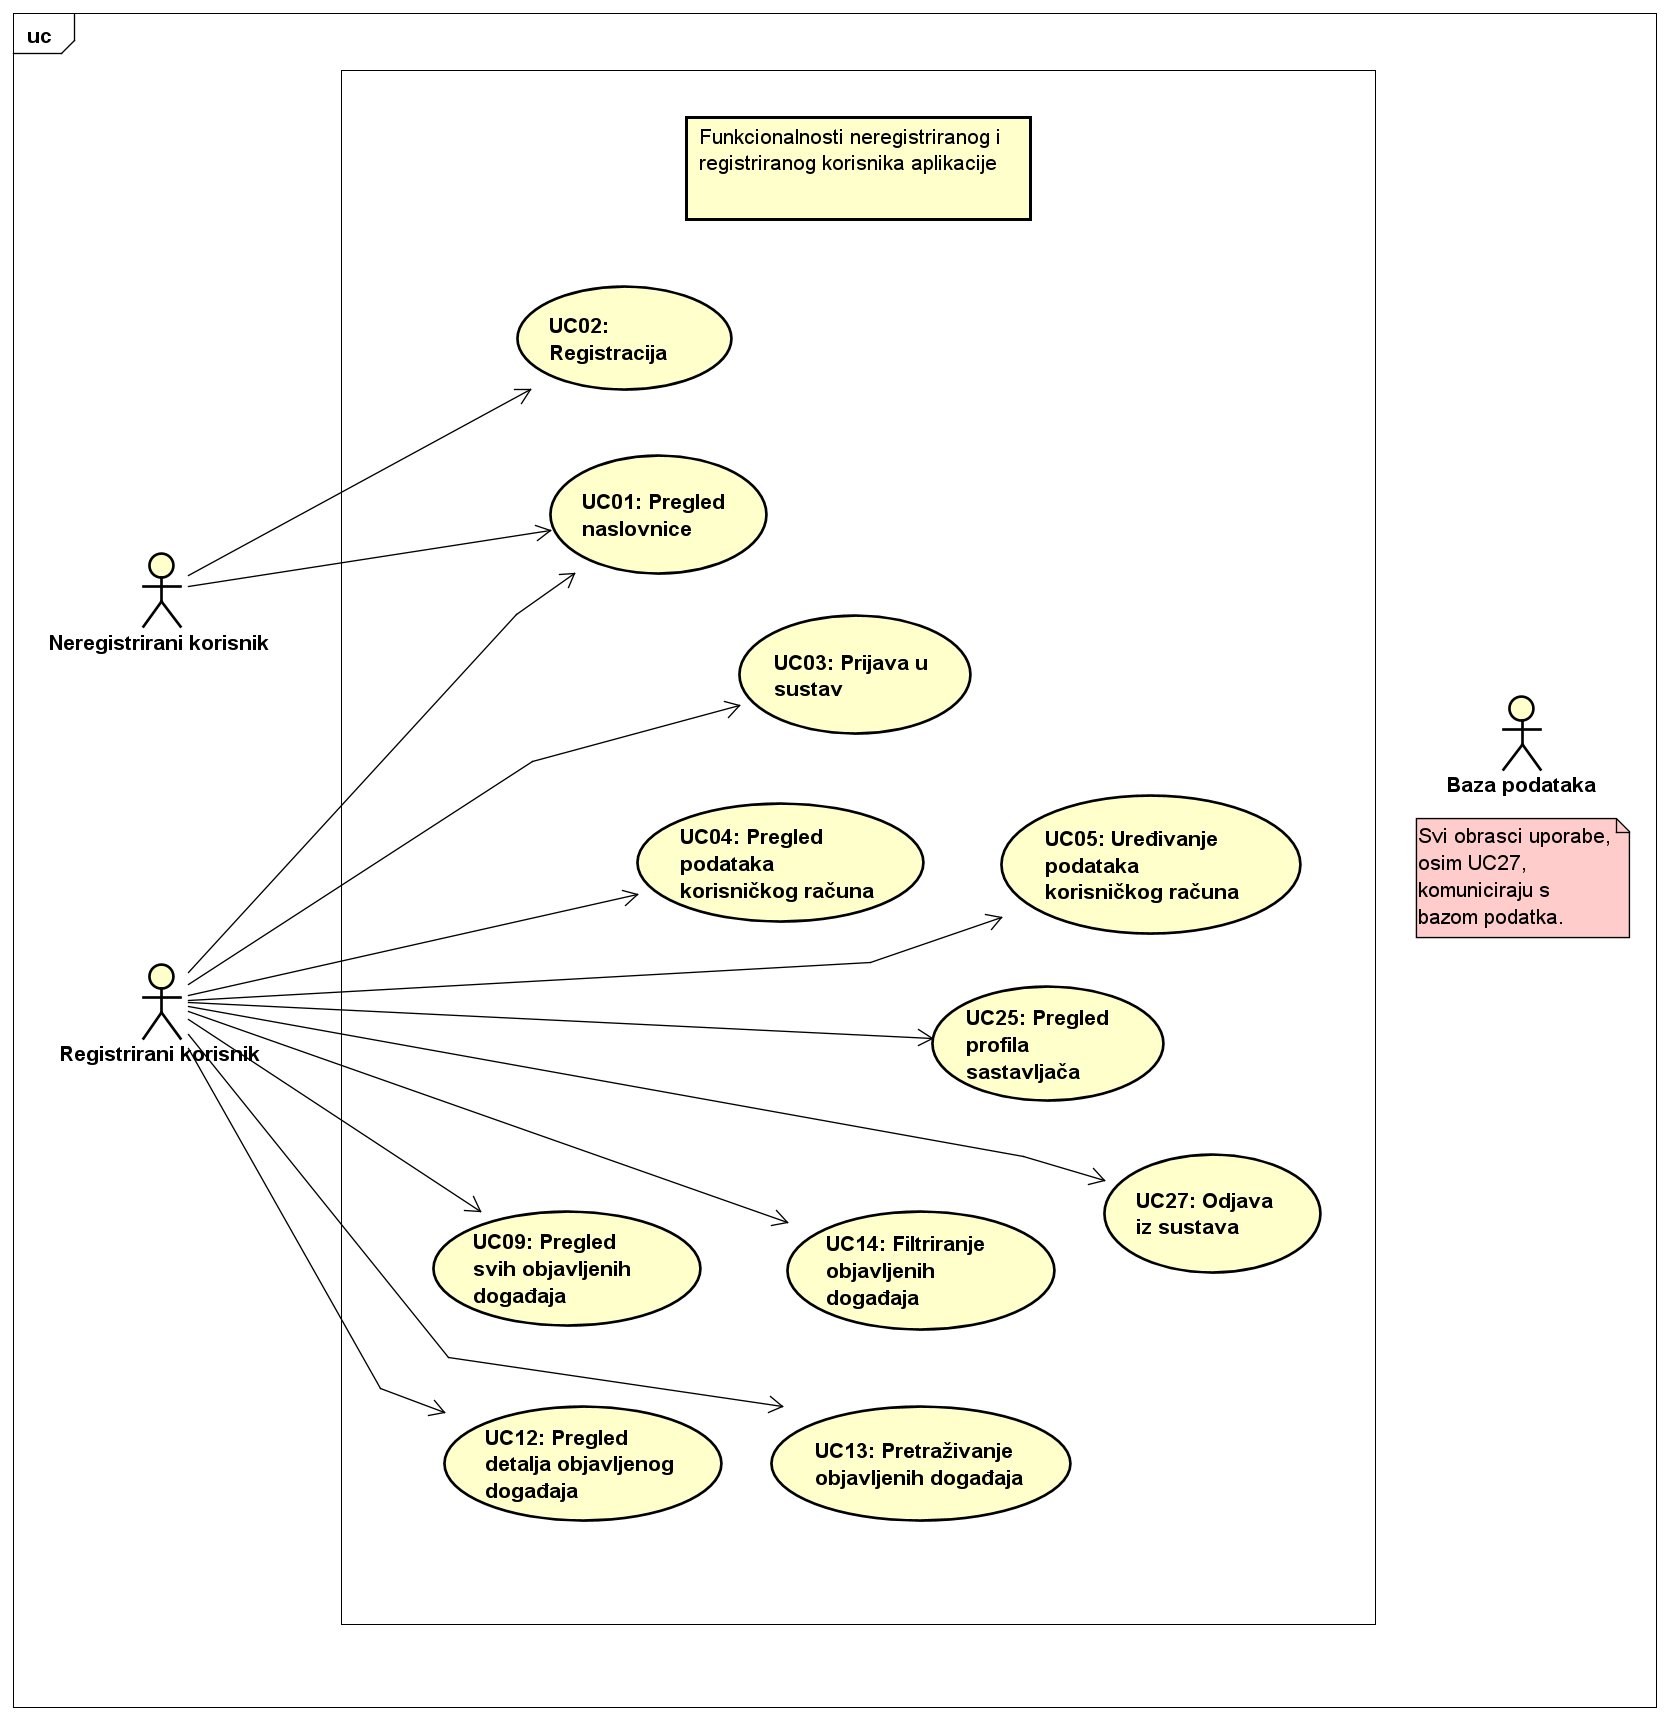
\includegraphics[width=\textwidth]{dijagrami/UseCaseDiagram1.PNG} 
					\caption{Dijagram obrazaca uporabe, funkcionalnosti neregistriranog i registriranog korisnika}
					\label{fig:UseCaseDiagram1}
				\end{figure}
				
				\begin{figure}[H]
					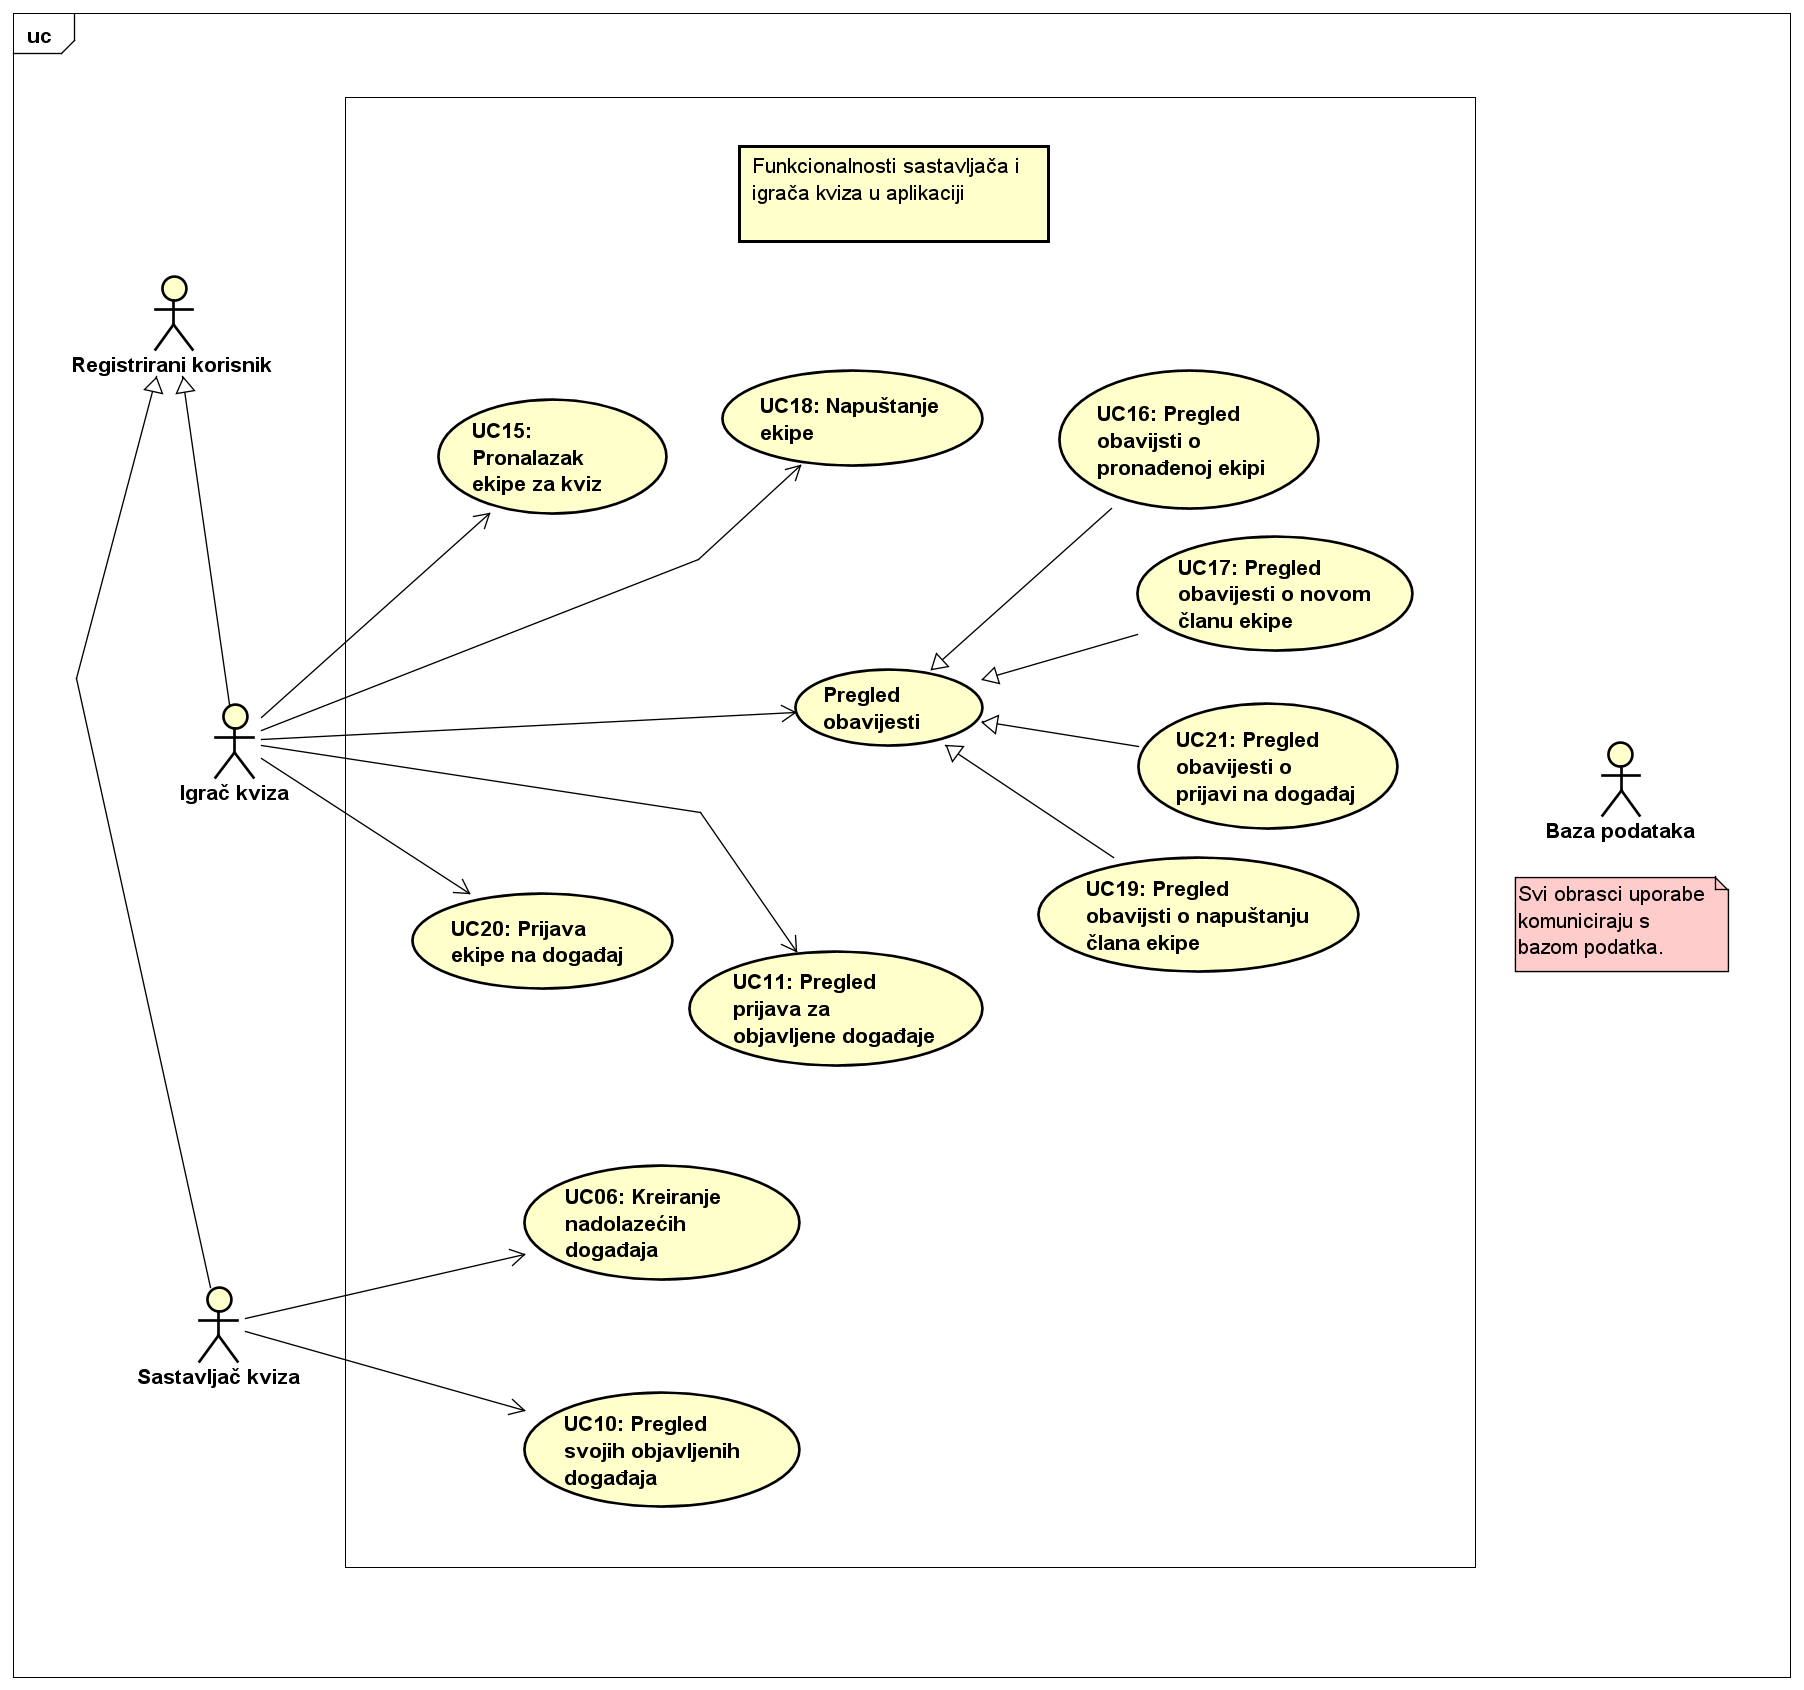
\includegraphics[width=\textwidth]{dijagrami/UseCaseDiagram2.PNG} 
					\caption{Dijagram obrazaca uporabe, funkcionalnosti igrača i sastavljača kviza}
					\label{fig:UseCaseDiagram2}
				\end{figure}
			
				\begin{figure}[H]
					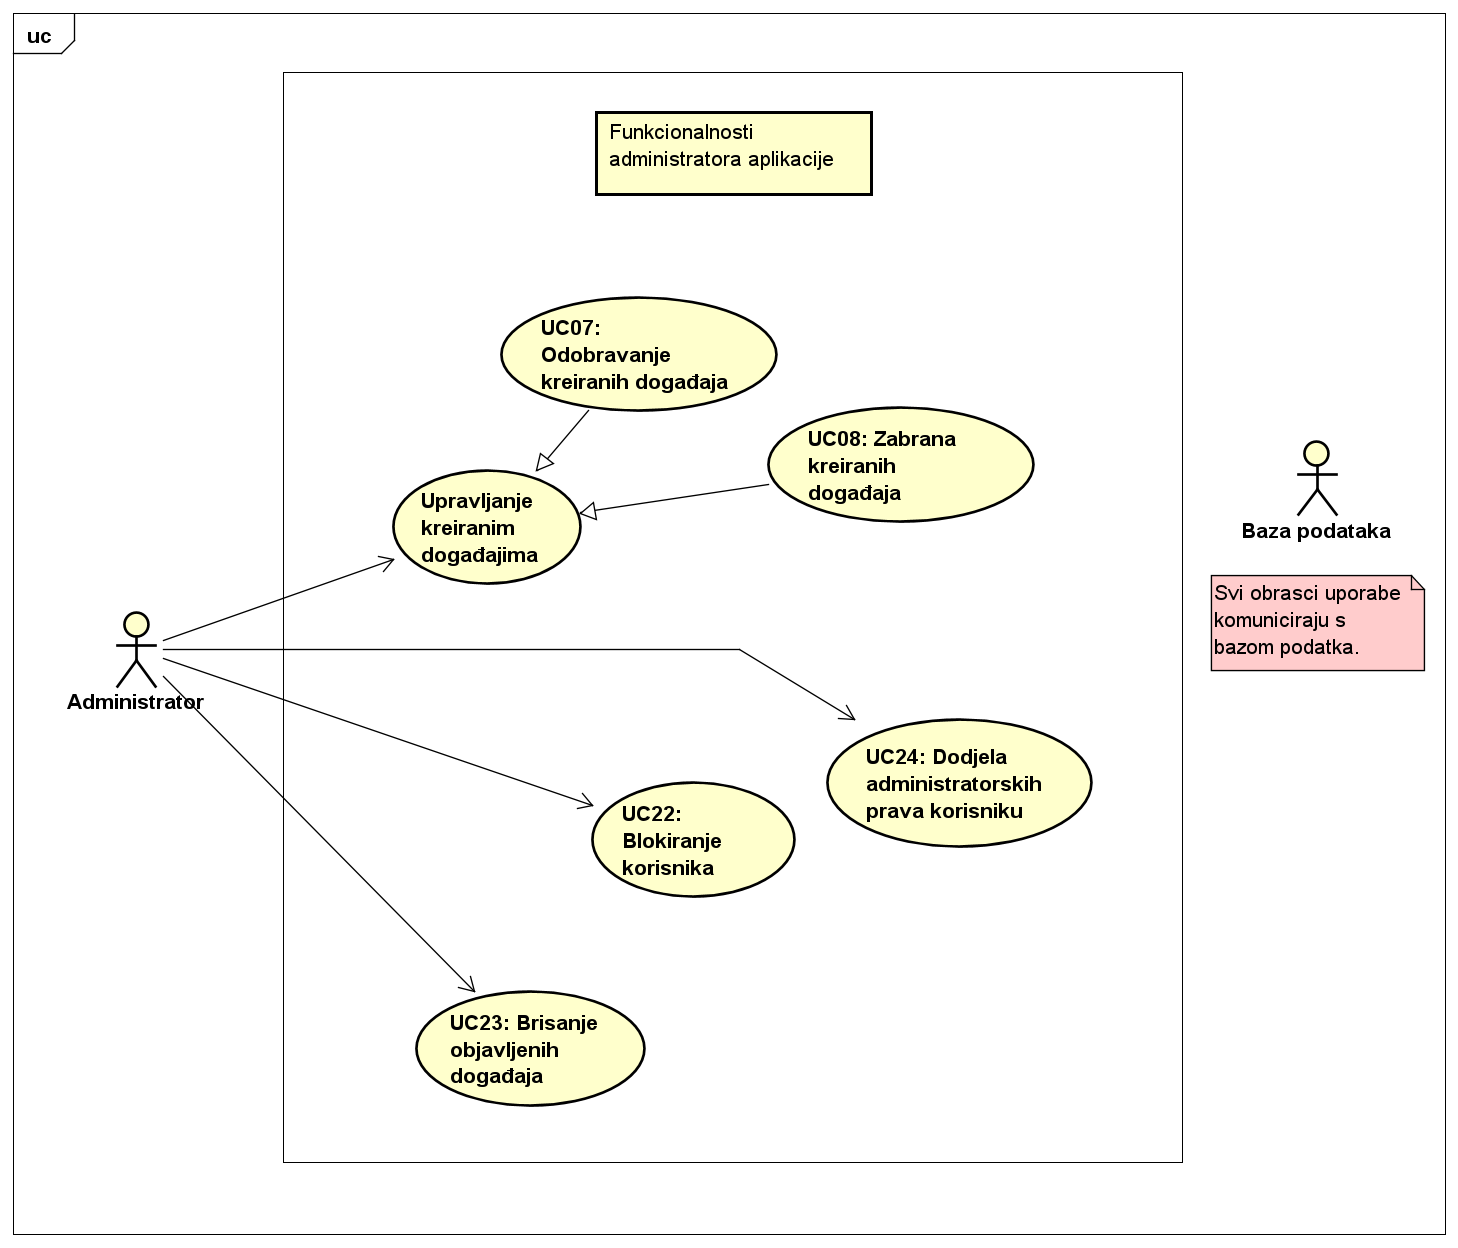
\includegraphics[width=\textwidth]{dijagrami/UseCaseDiagram3.PNG} 
					\caption{Dijagram obrazaca uporabe, funkcionalnosti administratora}
					\label{fig:UseCaseDiagram3}
				\end{figure}
				\eject		
				
			\subsection{Sekvencijski dijagrami}
				
				\textbf{\textit{dio 1. revizije}}\\
				
				\textit{Nacrtati sekvencijske dijagrame koji modeliraju najvažnije dijelove sustava (max. 4 dijagrama). Ukoliko postoji nedoumica oko odabira, razjasniti s asistentom. Uz svaki dijagram napisati detaljni opis dijagrama.}
				
				
				
				\begin{figure}[H]
					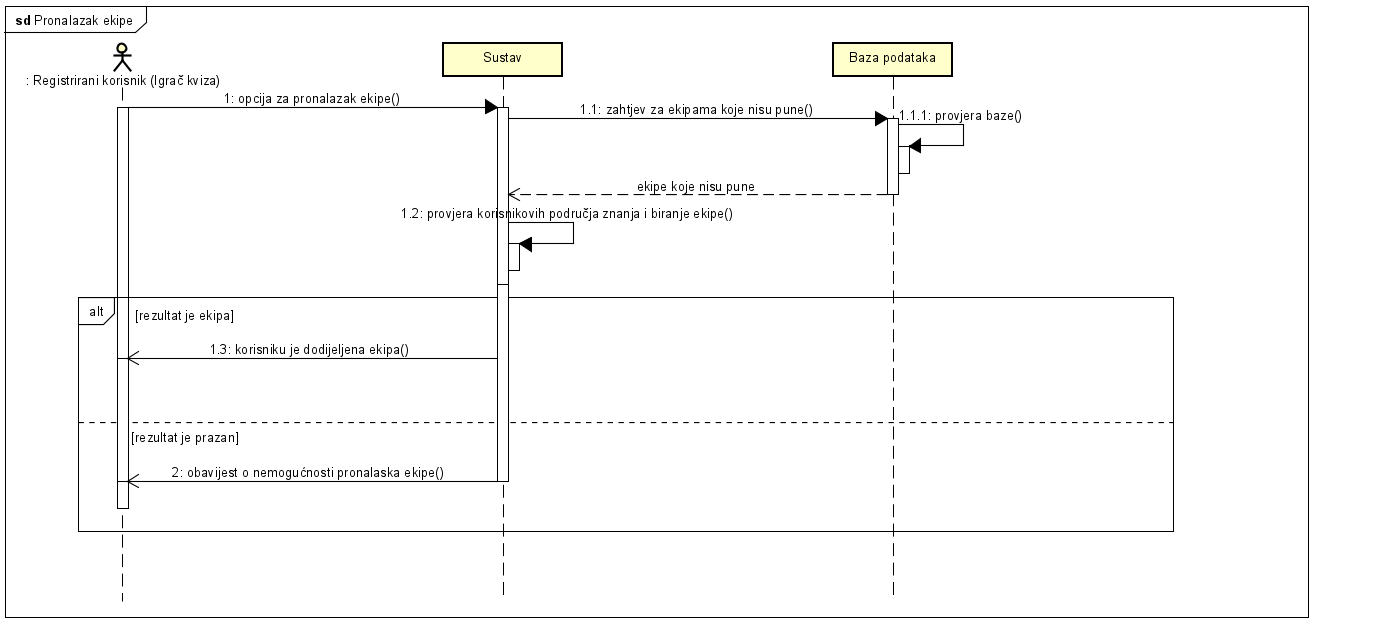
\includegraphics[width=\textwidth]{dijagrami/SeqDiagram3.PNG} 
					\caption{Sekvencijski dijagram, pronalazak ekipe}
					\label{fig:UseCaseDiagram3}
				\end{figure}

				\begin{figure}[H]
					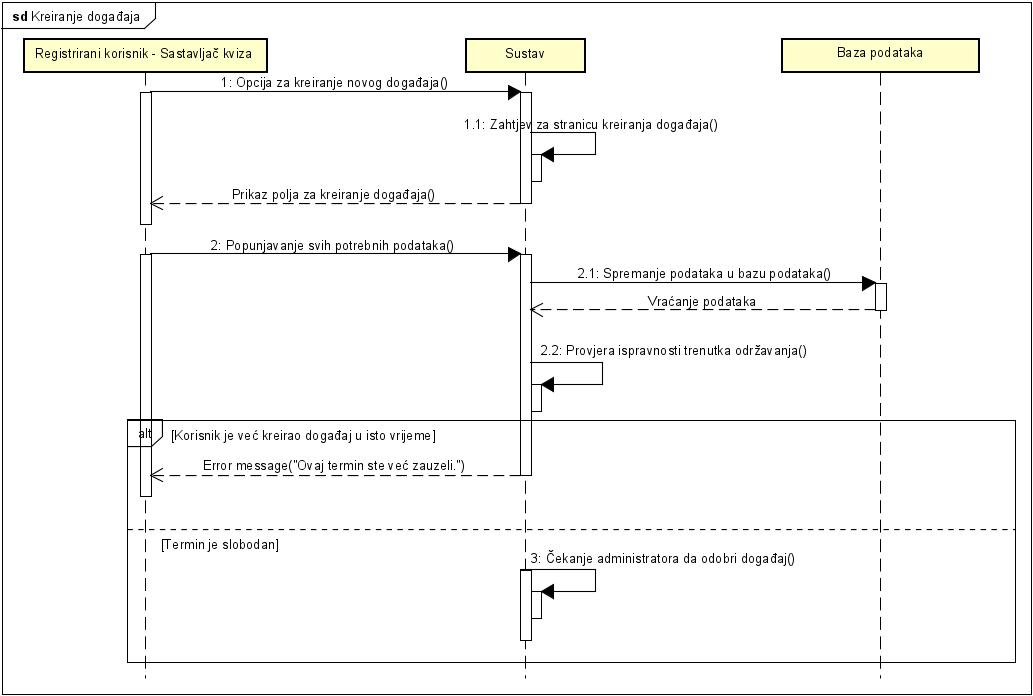
\includegraphics[width=\textwidth]{dijagrami/SekvencijskiKreiranjeDogadaja.PNG} 
					\caption{Sekvencijski dijagram, kreiranje događaja}
					\label{fig:UseCaseDiagram3}
				\end{figure}
				\eject

	
		\section{Ostali zahtjevi}
		
			\textbf{\textit{dio 1. revizije}}\\
		 
			 \textit{Nefunkcionalni zahtjevi i zahtjevi domene primjene dopunjuju funkcionalne zahtjeve. Oni opisuju \textbf{kako se sustav treba ponašati} i koja \textbf{ograničenja} treba poštivati (performanse, korisničko iskustvo, pouzdanost, standardi kvalitete, sigurnost...). Primjeri takvih zahtjeva u Vašem projektu mogu biti: podržani jezici korisničkog sučelja, vrijeme odziva, najveći mogući podržani broj korisnika, podržane web/mobilne platforme, razina zaštite (protokoli komunikacije, kriptiranje...)... Svaki takav zahtjev potrebno je navesti u jednoj ili dvije rečenice.}
			 
			 
			 
	